\documentclass[12pt,a4paper]{report}
\usepackage[left=3.00cm, right=2.00cm, top=2.00cm, bottom=2.00cm]{geometry}
\usepackage{vntex}
\usepackage{amsmath}
\usepackage{amssymb}
\usepackage{graphicx}
\author{LHD}
\newcommand{\nocontentsline}[3]{}
\newcommand{\tocless}[2]{\bgroup\let\addcontentsline=\nocontentsline#1{#2}\egroup}
\author{LHD}

\begin{document}
	\begin{center}
		BAN CƠ YẾU CHÍNH PHỦ\\
		\textbf{HỌC VIỆN KỸ THUẬT MẬT MÃ}
	\end{center}
\begin{figure}[h]
	\centering
	\includegraphics[width=0.25\linewidth]{"Pics/Logo HV"}
	\label{fig:logo-hv}
\end{figure}

\begin{center}
	ĐỀ CƯƠNG CHUYÊN ĐỀ AN TOÀN HỆ THỐNG THÔNG TIN\\
	\textbf{Nghiên cứu giải pháp đảm bảo an toàn cho Microservices trên Kubernetes}
\end{center}
\bigskip
\begin{flushright}
	Ngành: An toàn thông tin
\end{flushright}
\vspace{30mm}
\begin{flushleft}
	\textit{Sinh viên thực hiện:}\\
	\textbf{Phương Văn Sơn}\\
	Mã sinh viên: AT160258\\
	\textbf{Lê Huy Dũng}\\
	Mã sinh viên: AT160211
	\bigskip\\
	\textit{Người hướng dẫn:}\\
	\textbf{KS. Nguyễn Mạnh Thắng}\\
	Khoa An toàn thông tin - Học viện Kỹ thuật mật mã
\end{flushleft}
\vfill
\begin{center}
	Hà Nội, 2022
\end{center}

	\tableofcontents
	
	\chapter*{\centering Lời cảm ơn}
	\addcontentsline{toc}{chapter}{Lời cảm ơn}
	\hspace{1cm}Nhóm chúng em xin chân thành cảm ơn các thầy cô trường Học viện Kỹ thuật Mật mã nói chung, quý thầy cô của khoa An toàn thông tin nói riêng đã tận tình dạy bảo, truyền đạt kiến thức cho chúng em trong suốt quá trình học.\newline
	
	\hspace{1cm} Kính gửi đến Thầy Nguyễn Mạnh Thắng lời cảm ơn chân thành và sâu sắc nhất, cảm ơn thầy đã tận tình theo sát, chỉ bảo và hướng dẫn cho nhóm em trong quá trình thực hiện đề tài này. Thầy không chỉ hướng dẫn chúng em những kiến thức chuyên ngành, mà còn giúp chúng em học thêm những kĩ năng mềm, tinh thần học hỏi, thái độ khi làm việc nhóm.\\
	
	\hspace{1cm}Trong quá trình tìm hiểu nhóm chúng em xin cảm ơn các bạn sinh viên đã góp ý, giúp đỡ và hỗ trợ nhóm em rất nhiều trong quá trình tìm hiểu và làm đề tài.\\
	
	\hspace{1cm}Do kiến thức còn nhiều hạn chế nên không thể tránh khỏi những thiếu sót trong quá trình làm đề tài.Chúng em rất mong nhận được sự đóng góp ý kiến của quý thầy cô để đề tài của chúng em đạt được kết quả tốt hơn.\\
	\bigskip \\
	\textbf{Chúng em xin chân thành cảm ơn!}
	\chapter*{\centering Lời mở đầu}
	\addcontentsline{toc}{chapter}{Lời mở đầu}
	\hspace{1cm}{Nhiều năm trước, hầu hết các ứng dụng phần mềm đều được xây dựng với kiến trúc monolith hay còn gọi là kiến trúc 1 khối là mẫu thiết kế được dùng nhiều nhất trong giới lập trình web hiện nay bởi tính đơn giản của nó khi phát triển và khi triển khai. Các ứng dụng này chạy dưới dạng một tiến trình đơn lẻ hoặc số lượng nhỏ các tiến trình trên một số ít máy chủ. Chúng có khả năng cập nhật và nâng cấp chậm và yêu cầu nâng cấp thường xuyên. Trong trường hợp có sự cố như lỗi phần cứng hệ thống phần mềm này sẽ phải được di chuyển một cách thủ công sang các máy chủ còn hoạt động tốt.\\}
	
	{\hspace{0.3cm}Ngày nay các ứng dụng được xây dựng với kiến trúc lớn và phức tạp đang dần được chia thành các thành phần nhỏ hơn, có khả năng hoạt đông độc lập được gọi là microservices. Vì các Microservices tách biệt với nhau nên chúng có thể được phát triển, triển khai hay cập nhật và mở rộng quy mô một cách riêng lẻ. Nhờ khả năng này cho phép ta thay đổi các thành phần nhanh chóng và thường xuyên khi cần thiết để theo kịp với các yêu cầu thay đổi nhanh chóng thời nay.\\}
	
	\hspace{0.3cm}Nhưng với số lượng lớn các thành phần cũng như cơ sở dữ liệu việc cấu hình, quản lý và giữ hệ thống hoạt động trơn tru ngày càng trở nên khó khăn đặc biệt trong việc tối ưu hiệu quả sử dụng tài nguyên. Kubernetes ra đời ể đáp ứng nhu cầu tự động hoá như lập lịch tự động, cấu hình tự động hay giám sát và xử lý lỗi.\\
	
	\hspace{0.3cm}Kubernetes cung cấp cho các nhà phát triển khả năng triển khai các ứng dụng một cách thường xuyên mà không cần thông qua nhóm vận hành. Không chỉ dừng lại ở đó Kuberbetes cũng giúp nhóm vận hành tự động theo dõi và khắc phục sự cố. \\
	
	\hspace{0.3cm}Đi cùng với sự phát triển lớn mạnh của kiến trúc Microservices cũng như Kubernetes đó là nhu cầu về việc đảm bảo tính an toàn cho các hệ thống này. Trong bài báo cáo này chúng em sẽ giới thiệu về giải pháp đảm bảo an toàn cho Microservices bằng Istio Service Mesh
	
	\chapter{Giới thiệu về công nghệ Container và kiến trúc Microservices}
		\section{Giới thiệu về công nghệ Container}
		\section{Giới thiệu về kiến trúc Microservices}
		\section{Giới thiệu về Kubernetes}
				{\hspace{0.6cm}Kubernetes là một nền tảng nguồn mở quản lý các ứng dụng được đóng gói và các service, giúp thuận lợi trong việc cấu hình và tự động hoá việc triển khai ứng dụng.\\}
				
				Tên gọi Kubernetes có nguồn gốc từ tiếng Hy Lạp, có ý nghĩa là người lái tàu hoặc hoa tiêu. Google mở mã nguồn Kubernetes từ năm 2014. Kubernetes xây dựng dựa trên một thập kỷ rưỡi kinh nghiệm mà Google có được với việc vận hành một khối lượng lớn workload trong thực tế, kết hợp với các ý tưởng và thực tiễn tốt nhất từ cộng đồng.\\
			\subsection{Kiến trúc của Kubernetes}
				\begin{figure}[h]
					\centering
					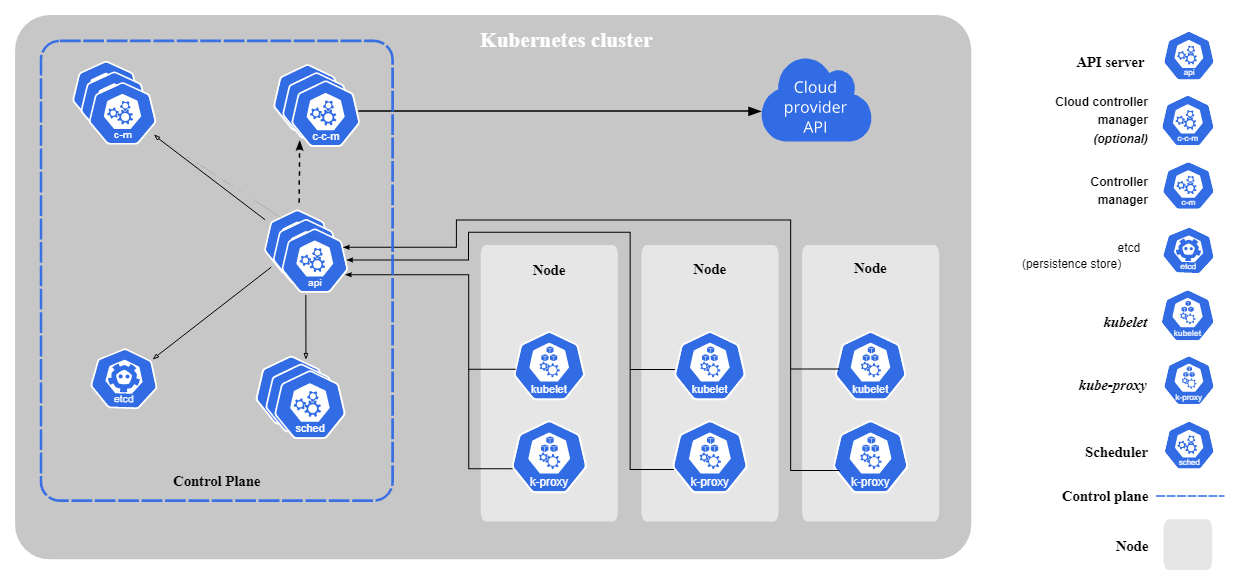
\includegraphics[width=0.7\linewidth]{Pics/kube-architecture}
					\caption{Kiến trúc của Kubernetes}
					\label{fig:kube-architecture}
				\end{figure}
			
				Các thành phần của cụm Kubernetes:\\
				
				\begin{itemize}				
					\item Control Plane: Là trung tâm điều khiển các cụm và làm các cụm kubernetes hoạt động. Đây là nơi quản lý, lên kế hoạch, lập lịch và theo dõi các pod, các node.
					\item Worker Node: Là một máy ảo hoặc máy vật lý chạy Kubernetes. Đây là nơi container thực sự được triển khai để chạy các ứng dụng.
				\end{itemize}
			
				{\hspace{0.3cm}Các thành phần của Control Plane:\\}
				
				\begin{itemize}				
					\item Kubernetes API server: Nơi mà các quản trị viên và các thành phần khác của Control Plane giao tiếp với nhau.
					\item Scheduler: lập lịch cho các ứng dụng của bạn (chỉ định các workload ví dụ như pods được triển khai ở worker node nào)
					\item  Controller Manager: thực hiện các chức năng cấp cụm, chẳng hạn như nhân bản các thành phần, theo dõi các node, xử lý các node lỗi,...
					\item etcd: một kho dữ liệu phân tán đáng tin cậy lưu trữ cấu hình của các node dưới dạng key value.
				\end{itemize}
			
				{\hspace{0.3cm}Các thành phần của Worker Node:\\}
				
				\begin{itemize}				
					\item kubelet: dùng để giao tiếp với API server và quản lý các container nằm trong node.
					\item kube-proxy: là một proxy chạy trên các node trong  Kubernetes. kube-proxy duy trì các quy tắc mạng trên các nút. Các quy tắc mạng này cho phép các Pods trong cùng một node hoặc khác node có thể giao tiếp với nhau.
					\item container-runtime: có thể là Docker, rkt, containerd hoặc một loại container-runtime khác.
				\end{itemize}
			
			\subsection{Tổng quan về Pod}
				{\hspace{0.6cm}Pod là đơn vị thực thi cơ bản của 1 ứng dụng Kubernetes, là đơn vị nhỏ nhất và đơn giản nhất trong mô hình object của Kubernetes. Một Pod đại diện cho các process (tiến trình) chạy trên cluster.\\}
				
				Pod đóng gói một container của ứng dụng (hoặc trong một số trường hợp là nhiều container), tài nguyên lưu trữ, một định danh network duy nhất (địa chỉ IP) cũng như các tùy chọn chi phối cách thức các container sẽ chạy. Một Pod đại diện cho một đơn vị triển khai: một instance (phiên bản) của một ứng dụng trong Kubernetes, có thể chứa một container hoặc vài container được liên kết chặt chẽ và chia sẻ tài nguyên.\\
				
				Docker là container runtime phổ biến nhất được sử dụng cho Pod trong Kubernetes, tuy nhiên Pods cũng hỗ trợ các container runtime khác.\\
				
				Pod trong Kubernetes cluster có thể được sử dụng theo hai cách chính:\\
				\begin{itemize}				
					\item Pods chạy một container duy nhất. Mô hình “một-container-một-Pod” là trường hợp sử dụng phổ biến nhất của Kubernetes; trong trường hợp này, ta có thể nghĩ về một Pod như một trình bao bọc (đóng gói) xung quanh một container và Kubernetes quản lý các Pod thay vì quản lý trực tiếp các container.
					\item Pods chạy nhiều container cần tương tác với nhau. Một Pod có thể đóng gói một ứng dụng chứa nhiều container cùng hoạt động và được liên kết chặt chẽ với nhau cũng như cần chia sẻ tài nguyên (được gọi là co-located container). Các co-located container này có thể tạo thành một đơn vị dịch vụ gắn kết duy nhất nghĩa là 1 container phục vụ các file từ một volume chia sẻ cho public, trong khi đó, một “sidecar” container khác sẽ làm mới (refresh) hoặc cập nhật các file đó. Pod đóng gói các container và tài nguyên lưu trữ này lại với nhau như một thực thể có thể quản lý được.
				\end{itemize}
			\subsection{Vòng đời của Pod}
				{\hspace{0.6cm}Giống như các container, Pod được coi là các thực thể tạm bợ, không bền vững(thay vì lâu bền). Các Pod được tạo, gán một ID (UID) duy nhất và được lên lịch cho các node mà chúng vẫn duy trì cho đến khi bị hủy bỏ (theo chính sách khởi động lại) hoặc xóa. Nếu một node chết, các Pod được lập lịch cho node đó sẽ được lập lịch để xóa sau một khoảng thời gian chờ.\\}
				
				Pod không tự chữa lành. Nếu một Pod được lên lịch cho một node sau đó không thành công, Pod đó sẽ bị xóa; tương tự như vậy, một Pod sẽ không tồn tại sau khi bị trục xuất do thiếu tài nguyên hoặc bảo trì Node. Kubernetes sử dụng phần trừu tượng cấp cao hơn, được gọi là bộ điều khiển, xử lý công việc quản lý các cá thể Pod tương đối dùng một lần.\\
				
				Một Pod nhất định (như được xác định bởi UID) không bao giờ được "lên lịch" đến một nút khác; thay vào đó, Pod đó có thể được thay thế bằng một Pod mới, gần giống, thậm chí có cùng tên nếu muốn, nhưng với một UID khác.\\
				
				Giai đoạn của Pod là một bản tóm tắt đơn giản về vị trí của Pod trong vòng đời của nó.Các giai đoạn của Pod:
				\begin{itemize}				
					\item Pending: Pod đã được chấp nhận bởi hệ thống kubernetes, nhưng 1 hoặc vài container image chưa được tạo ra. Nó bao gồm thời gian trước khi được lập lịch cũng như thời gian download image trên mạng về (có thể mất một lúc)
					\item Running: Pod đã được đưa vào 1 node và tất cả các container đã được tạo ra. Ít nhất 1 container vẫn đang chạy hoặc đang ở trong quá trình bắt đầu hoặc khởi động lại.
					\item  Succeeded: Tất cả các container trong pod đã kết thúc thành công và sẽ không được khởi động lại nữa.
					\item  Failed: Tất cả các container trong pod đã kết thúc và ít nhất 1 contrainer đã thất bại trong quá trình kết thúc. Có nghĩa là container đã exited (thoát) với trạng thái non-zero hoặc đã bị kết thúc bởi hệ thống.
					\item  Unknown: Vì một số lý do, trạng thái của pod không thể xác định được, thường là do bị lỗi trong việc giao tiếp với host của pod.
				\end{itemize}
			\subsection{Quản lí pod bằng Workload trên Kubernetes}
				{\hspace{0.6cm}Workload là một ứng dụng chạy trên Kubernetes. Cho dù workload là một thành phần đơn lẻ hay nhiều thành phần hoạt động cùng nhau, trên Kubernetes, chúng chạy bên trong một tập hợp các pod. Trong Kubernetes, Pod đại diện cho một tập hợp các container đang chạy trên cụm của bạn.\\}
				
				Các Pod có một vòng đời xác định. Ví dụ: khi một Pod đang chạy trong cụm thì một lỗi nghiêm trọng trên node nơi pod đó đang chạy có nghĩa là tất cả các pod trên node đó đều bị lỗi. Kubernetes coi mức độ thất bại đó là cuối cùng: bạn sẽ cần tạo một Pod mới để khôi phục, ngay cả khi node sau đó trở lại bình thường.\\
				
				Tuy nhiên, để làm cho công việc dễ dàng hơn, chúng ta không cần phải quản lý trực tiếp từng Pod. Thay vào đó, bạn có thể sử dụng các workload để quản lý một nhóm các Pod. Các tài nguyên này định cấu hình bộ điều khiển để đảm bảo số lượng phù hợp của loại Pod phù hợp đang chạy, phù hợp với trạng thái chúng ta đã cấu hình.\\
				
				Kubernetes cung cấp một số workload tích hợp sẵn:
				\begin{itemize}				
					\item Deployment và ReplicaSet (thay thế cho ReplicationController). Deployment rất phù hợp để quản lý workload không trạng thái trên cụm, nơi bất kỳ Pod nào trong Deployment đều có thể hoán đổi cho nhau và có thể được thay thế nếu cần.
					\item StatefulSet là workload API object được dùng để quản lý các ứng dụng stateful (có trạng thái). Nó quản lý việc triển khai và co giãn (scale) các pod và cung cấp sự đảm bảo về thứ tự và tính duy nhất của các pod này.
					\item  Một DeamonSet đảm bảo rằng tất cả hoặc một vài node sẽ chạy 1 bản sao của pod. Khi các node được thêm vào cluster thì pod sẽ được lập lịch vào chúng.
					\item  Job và CronJob xác định các nhiệm vụ chạy đến khi hoàn thành và sau đó dừng lại. Công việc đại diện cho các nhiệm vụ một lần, trong khi CronJobs lặp lại theo lịch trình.
				\end{itemize}
		\section{Một số vấn đề bảo mật kiến trúc Microservices}
			{\hspace{0.6cm}Trong hầu hết các ứng dụng được xây dựng trên cấu trúc monolith, bảo mật được thực thi tập trung và các thành phần riêng lẻ không cần phải lo lắng về việc thực hiện các kiểm tra bảo mật trừ khi có yêu cầu. Kết quả là, mô hình bảo mật của một ứng dụng dựa trên cấu trúc monolith là đơn giản hơn nhiều so với ứng dụng được xây dựng dựa trên cấu trúc microservices. Sau đây là một số vấn đề về bảo mật của kiến trúc Microservices gặp phải.\\}			
			\subsection{Càng nhiều microservices thì nguy cơ bị tấn công càng cao}
				{\hspace{0.6cm}Trong một ứng dụng được xây dựng trên cấu trúc monolith, giao tiếp giữa các thành phần bên trong xảy ra trong một tiến trình duy nhất — ví dụ: trong một ứng dụng Java, trong cùng một Máy ảo Java (JVM). Theo kiến trúc microservices, các thành phần bên trong đó được thiết kế dưới dạng các microservices riêng biệt, độc lập và các tiến trình phải gọi lẫn nhau để trao đổi các thông tin. Ngoài ra, mỗi microservice hiện chấp nhận các request một cách độc lập hoặc có các điểm truy cập riêng. Thay vì một vài điểm truy cập, như trong một ứng dụng xây dựng trên cấu trúc monolith, bây giờ chúng ta có số lượng lớn các điểm truy cập. Khi số lượng truy cập vào hệ thống tăng lên, chúng ta sẽ có nhiều điểm bị tấn công hơn. Vấn đề này là một trong những thách thức cơ bản trong việc xây dựng thiết kế bảo mật cho microservices.\\}
			\subsection{Kiểm tra bảo mật phân tán có thể dẫn đến hiệu suất giảm}
				{\hspace{0.6cm}Không giống như trong một ứng dụng được xây dựng trên cấu trúc monolith, mỗi microservice trong triển khai microservices phải thực hiện kiểm tra an ninh độc lập. Từ quan điểm của một ứng dụng dựa trên cấu trúc monolith, trong đó việc kiểm tra bảo mật được thực hiện một lần và các request được gửi đến thành phần tương ứng, nhưng đối với các microservice chúng ta phải kiểm tra tất các các điểm truy cập của chúng. Ngoài ra, trong khi xác thực các yêu cầu tại mỗi microservice, bạn có thể cần kết nối với dịch vụ mã thông báo bảo mật từ xa (STS). Các kiểm tra bảo mật phân tán, lặp đi lặp lại và kết nối từ xa này có thể làm tăng độ trễ và làm giảm đáng kể hiệu suất của hệ thống.\\}
				
				Một số giải quyết vấn đề này bằng cách đơn giản là tin tưởng vào mạng và tránh kiểm tra bảo mật các microservice. Theo thời gian, mạng tin cậy đã trở thành lỗi thời và đang tiến tới các nguyên tắc mạng không tin cậy. Với nguyên tắc mạng không tin cậy, chúng ta thực hiện bảo mật với từng tài nguyên trong mạng. Mọi thiết kế bảo mật microservices phải có hiệu suất tổng thể có thể chấp nhận được.
			\subsection{Sự phức tạp khi triển khai xác thực khởi động giữa các	microservices}
				{\hspace{0.6cm}Giao tiếp dịch vụ với dịch vụ diễn ra giữa các microservice. Mỗi kênh liên lạc giữa các microservice phải được bảo vệ. Chúng có nhiều tùy chọn, nhưng giả sử rằng chúng ta sử dụng chứng chỉ (certificates).\\}
				
				Giờ đây, mỗi microservice phải được cấp chứng chỉ (và khóa bí mật tương ứng), chứng chỉ này sẽ sử dụng để xác thực chính nó với một microservice khác trong quá trình tương tác giữa dịch vụ với dịch vụ. Microservice của người nhận phải biết cách xác thực chứng chỉ được liên kết với microservice đang gọi. Do đó cần một cách để tin tưởng bootstrap giữa các microservices. Ngoài ra cần có khả năng thu hồi chứng chỉ (trong trường hợp khóa bí mật tương ứng bị xâm phạm) và cấp các chứng chỉ mới (thay đổi chứng chỉ định kỳ để giảm thiểu mọi rủi ro khi vô tình làm mất chìa khóa). Những tác vụ này rất cồng kềnh và trừ khi chúng ta tìm ra cách tự động hóa chúng.\\
			\subsection{Khó theo dõi các request của các microservice}
				{\hspace{0.6cm}Khả năng giám sát là thước đo những gì có thể suy ra về trạng thái bên trong của một hệ thống dựa trên kết quả đầu ra bên ngoài của nó. Nhật ký (logs), chỉ số (metrics) và dấu vết (traces) được coi là ba trụ cột của khả năng giám sát.\\}
				
				Nhật ký có thể là bất kỳ sự kiện nào bạn ghi lại tương ứng với một dịch vụ nhất định.\\
				
				Tổng hợp một tập hợp các nhật ký có thể tạo ra các chỉ số. Theo một cách nào đó, các chỉ số phản ánh trạng thái hệ thống. Ví dụ về mặt bảo mật, các yêu cầu truy cập không hợp lệ trung bình mỗi giờ là một chỉ số.\\
				
				Dấu vết cũng dựa trên nhật ký nhưng cung cấp một góc nhìn khác về hệ thống. Theo dõi giúp bạn theo dõi một yêu cầu từ điểm mà nó đi vào hệ thống đến chỉ nơi nó rời khỏi hệ thống. Quá trình này trở nên khó khăn trong mô hình microservices. Không giống như trong một ứng dụng theo cấu trúc monolith, một yêu cầu triển khai microservices có thể xâm nhập vào hệ thống thông qua một microservice và trải dài trên nhiều microservices trước khi nó rời khỏi hệ thống.			
			\subsection{Tính bất biến của container làm việc xác thực và chính sách kiểm soát truy cập của các dịch vụ khó khăn}
				{\hspace{0.6cm}Máy chủ không thay đổi trạng thái sau khi quay được gọi là máy chủ bất biến. Các mô hình triển khai phổ biến nhất cho microservices là dựa trên container. Mỗi microservice chạy bằng container riêng của nó và tất nhiên, container phải là một máy chủ bất biến. Nói cách khác, sau khi container khởi động, nó sẽ không thay đổi bất kỳ tệp nào trong hệ thống tệp của nó hoặc duy trì bất kỳ trạng thái của nó không thay đổi lúc nó đang chạy.\\}
				
				Tính bất biến có tác động gì đến bảo mật và tại sao khái niệm máy chủ bất biến lại được coi là thách thức bảo mật microservices? Trong kiến trúc bảo mật microservices, mỗi microservice trở thành một điểm cần được bảo mật. Do đó, cần duy trì danh sách các máy khách được phép (có thể là các microservice khác) có thể truy cập vào microservice này và cần một bộ chính sách kiểm soát truy cập. Những danh sách này không tĩnh; chúng ta cần được phép cập nhật các danh sách này. Nhưng với tính chất bất biến của container, chúng ta không thể update hệ thống tệp trong các container của các microservice.
			\subsection{Kiến trúc đa ngôn ngữ đòi hỏi các developer phải có thêm nhiều kiến thức bảo mật hơn}
				{\hspace{0.6cm}Trong triển khai microservices, các dịch vụ nói chuyện với nhau qua mạng. Họ không phụ thuộc vào việc triển khai từng dịch vụ, mà phụ thuộc vào giao diện dịch vụ. Tình huống này cho phép mỗi microservice chọn ngôn ngữ lập trình của riêng mình và nền tảng công nghệ để triển khai. Trong một môi trường, trong đó mỗi đội development triển khai các mircoservice của riêng mình, mỗi nhóm có thể linh hoạt để chọn các stack công nghệ để phù hợp với sản phẩm. Kiến trúc này, cho phép các các thành phần trong hệ thống để chọn công nghệ tốt nhất cho chúng, được gọi là một kiến trúc đa ngôn ngữ.\\}
				
				Một kiến trúc đa ngôn ngữ làm cho vấn đề bảo mật trở nên khó khăn. Bởi vì các đội khác nhau sử dụng các stack công nghệ khác nhau để phát triển, mỗi nhóm phải có các chuyên gia bảo mật riêng. Các chuyên gia này phải chịu trách nhiệm xác định các phương pháp bảo mật tốt nhất và hướng dẫn, nghiên cứu các công cụ bảo mật cho mỗi stack công nghệ để phân tích mã nguồn tĩnh và thử nghiệm động và tích hợp các công cụ đó vào quá trình xây dựng. Trách nhiệm của một nhóm bảo mật tập trung, nhưng bây giờ chia vào các đội development. Điều này làm cho các đội development không chú tâm vào việc phát triển sản phẩm mà phải lo một phần về bảo mật nữa làm cho chất lượng sản phẩm giảm do phải viết các module bảo mật làm cho mã nguồn bị rối và khó đọc.
				
				
		\section*{Kết luận Chương 1}
	
	\chapter{Tổng quan về Istio}
		\section{Tổng quan về Istio}
			\subsection{Tổng quan về Service Mesh}
			\subsection{Kiến trúc của Istio}
		\subsection{Tổng quan về Envoy Proxy}
		\section{Quản lý mạng giữa các Microservices với Istio}
			\subsection{Tổng quan về Istio Ingress Gateway}
			\subsection{Định tuyến trong Istio}
			\subsection{Giải quyết các vấn đề về mạng trong Microservices}
		\section{Giám sát các Microservices với Istio}
			\subsection{Một số Metrics quan trọng của Istio}
			\subsection{Giám sát các lưu lượng mạng qua Jaeger và Kiali}
		\section{Bảo mật các Microservices bằng Istio}
			\subsection{Xác thực giữa các Microservices với Istio}
			\subsection{Phân quyền cho các Microservices với Istio}
		\section*{Kết luận chương 2}
	\chapter{Triển khai Istio trên Kubernetes}
		\section{Mô hình triển khai}
		\section{Kịch bản triển khai}
		\section{Thực nghiệm}
		\section{Kết luận}
	
\end{document}